\documentclass[a4paper]{article}

\usepackage[english]{babel}
\usepackage[utf8x]{inputenc}
\usepackage{amsmath}
\usepackage{graphicx}
\usepackage[colorinlistoftodos]{todonotes}
\usepackage[margin=1in]{geometry}
\usepackage{listings}
\usepackage{xcolor}
\usepackage{cascadia-code}
\usepackage{animate}
\usepackage{subfigure}
\usepackage{float}
\newcommand{\dotr}[1]{#1^{\bullet}} 
\definecolor{codegreen}{rgb}{0,0.6,0}
\definecolor{codegray}{rgb}{0.5,0.5,0.5}
\definecolor{codepurple}{rgb}{0.58,0,0.82}
\definecolor{backcolour}{rgb}{0.95,0.95,0.92}

\usepackage{tabularx}
\lstdefinestyle{mystyle}{
    backgroundcolor=\color{backcolour},   
    commentstyle=\color{codegreen},
    keywordstyle=\color{magenta},
    numberstyle=\tiny\color{codegray},
    stringstyle=\color{codepurple},
    basicstyle=\ttfamily\footnotesize,
    breakatwhitespace=false,         
    breaklines=true,                 
    captionpos=b,                    
    keepspaces=true,                 
    numbers=left,                    
    numbersep=5pt,                  
    showspaces=false,                
    showstringspaces=false,
    showtabs=false,                  
    tabsize=2
}
\lstset{style=mystyle}
\title{Northeastern University\\EECE 5554 Robotics Sensing and Navigation \\ Lab 2 submission}
\author{Yash Mewada}
\date{Feb 21, 2023}

\begin{document}
\maketitle
\section{A brief introduction to ArduSimple SimpleRTK2B modules.}
We learned in the previous Lab that standard GPS modules have no differential method of knowing whether the received data is true or not. That is why we got significant values of RMSE. The RTK is made to minimize this error by using two GPS modules and performing Real Time Kinematics. A simple setup consists of a Base and a Rover. The Base receives the GPS data from the satellite, this data consists of \textbf{Ephimeris data - Orbital Position of the satellite} as well as the Latitude and Longitude of the Base. Due to environmental and architectural reasons, there is always an error in these data. \\
\textit{When a transformation is done on the ephemeris data to project it in the 2D plane we get Lat and Long.} \\
The base performs the above calculations and sends the corrections of these errors to the rover. The rover then uses these corrections to display a more accurate and precise location.\\
In general, the RTK modules have an accuracy of 5cm - 10cm and a precision of around 0.5cm - 1cm.\\
\begin{figure}[h]
    \centering
    \includegraphics[scale = 0.2]{setup.jpg}
    \caption{simpleRTK2B - Starter Kit LR}
    \label{fig:simpleRTK2B - Starter Kit LR}
\end{figure}
The above figure resembles our setup.\\
\begin{enumerate}
    \item 2x simpleRTK2B boards with Ublox F9P controllers
    \item 2x Xbee SiF 915MHz LoRa (Long Range) modules with telemetry radios
    \item 2x GNSS Mulitband antennas
\end{enumerate}
The two SimpleRTK boards communicate with each other via an XBee LoRa module. The base is generally stationary and sends the data to the rover. This specific setup had a range of 10km (within line of sight) between Rover and Base and 2.5km - 5km with a partial line of sight. The lowered frequency (\textbf{915 MHZ}) is what makes them Long Range.\\
\section{How to quantify the quality of GPS data.}
As mentioned above, the base collects the \textit{Ephimeris} data of the satellite and performs the corrections. Initially, with GPS Puck, the fixed quality indicator was 1 - GPS fix i.e just getting the signal from satellites.\\ The base station uses \textbf{Precision Orbit Determination (POD)} to determine the position of the satellite at a sub-centimeter level of accuracy. This is basically performing a coordinate transformation of the satellite's orbital location i.e \textbf{World geodetic system 1984 (WGS84)} to a 2D plane of UTM or Latitude and Longitude. Now the base has measurements and the satellite's location and can perform RTK based on it and send those corrections to the rover.\\ As the rover receives these corrections, it finds a proper combination of signals from satellites and base correction to accurately determine its own position. As the rover finds this combination the fixed quality changes to \textbf{\textit{RTK Fixed - 4}}.\\
These position estimates are computed continuously and instantaneously, as the GPS measurements are received hence \textbf{Real Time }. RTK is also called \textbf{kinematic} because it is based on the principles of kinematics, which is the study of motion without considering the forces that cause the motion. 
\section{GNSS with RTK vs without}
Below is the scatterplot of UTM-Northing vs UTM-Easting for different datasets.
\begin{figure}[h]
\begin{subfigure}{}
     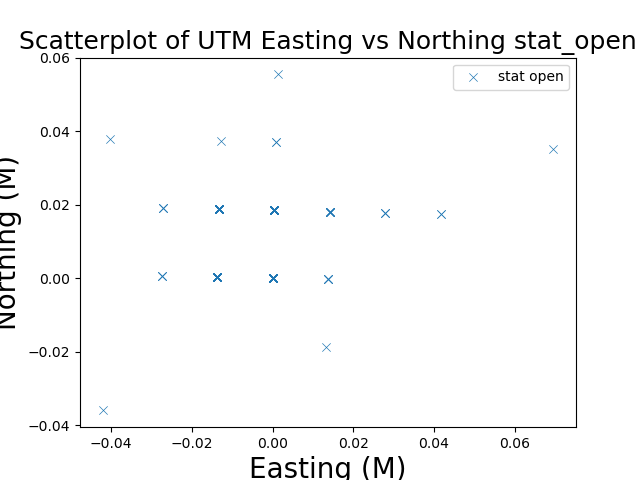
\includegraphics[scale = 0.3]{plot-Scatterplot of UTM Easting vs Northing stat_open.png}
\end{subfigure}
\begin{subfigure}{}
    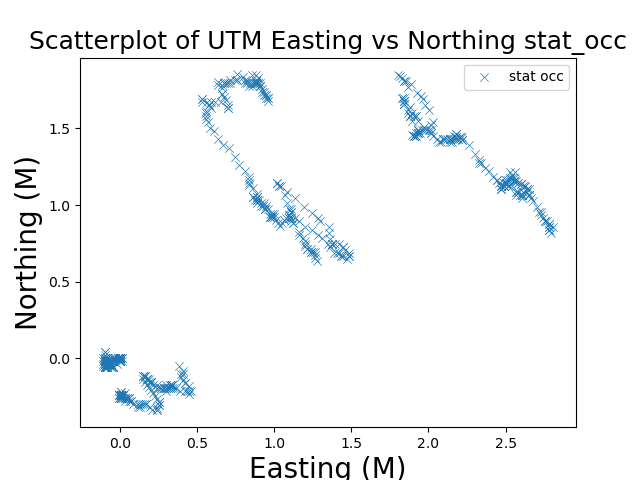
\includegraphics[scale = 0.3]{plot-Scatterplot of UTM Easting vs Northing stat_occ.png}
\end{subfigure}
\begin{subfigure}{}
    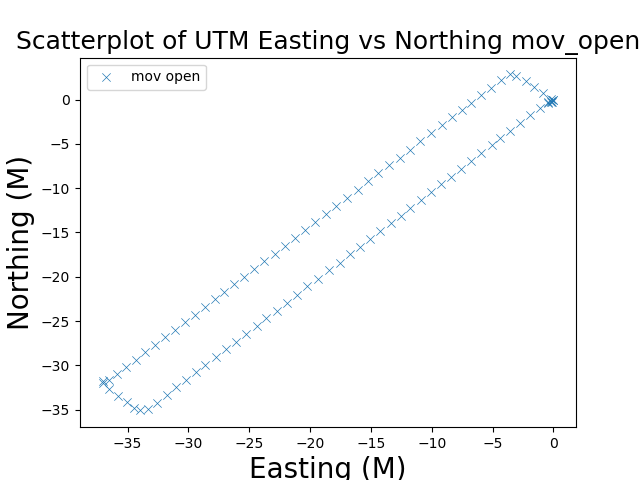
\includegraphics[scale = 0.3]{plot-Scatterplot of UTM Easting vs Northing mov_open.png}
\end{subfigure}
\begin{subfigure}{}
    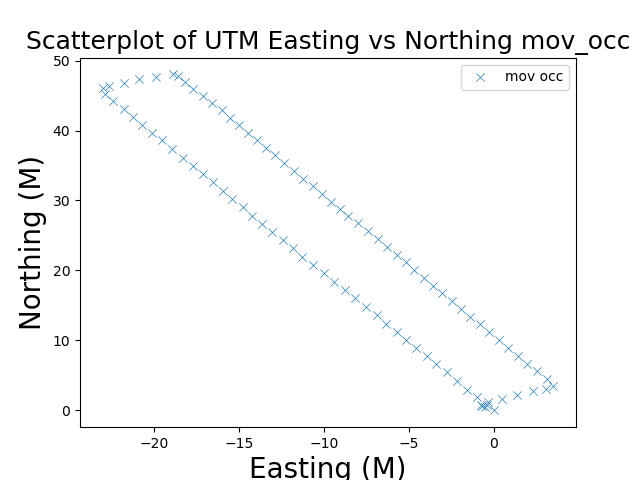
\includegraphics[scale = 0.3]{plot-Scatterplot of UTM Easting vs Northing mov_occ.png}
\end{subfigure}
\caption{UTM Easting vs UTM Northing Scatterplots.}
\label{Fig 1: UTM Easting vs UTM Northing Scatterplots.}
\end{figure}
\textbf{\textit{RMSE from known open position - 0.000612}}.\\
The errors in the above graphs make sense based on the locations it was taken.
Columbus Garage for Stationary Open and Squash Busters for Stationary Occluded. Carter field for walking open and Robbinson Hall for walking occluded. \textbf{The base was in the same position for all data collection i.e on top of Columbus Garage.}\\
The deviation of the data from the above graphs tells us that RTK-based GPS is more sensitive to the movements of the rover/base. As they tend to have an accuracy of 5-10cm. Furthermore, it tells us that without RTK the data was more deviated whereas with RTK this densely packed data (especially for stationary open) shows us better accuracy of the module.
\section{Distribution of error}
Below are the histograms for the stationary datasets.
\begin{figure}[h]
\begin{subfigure}{}
     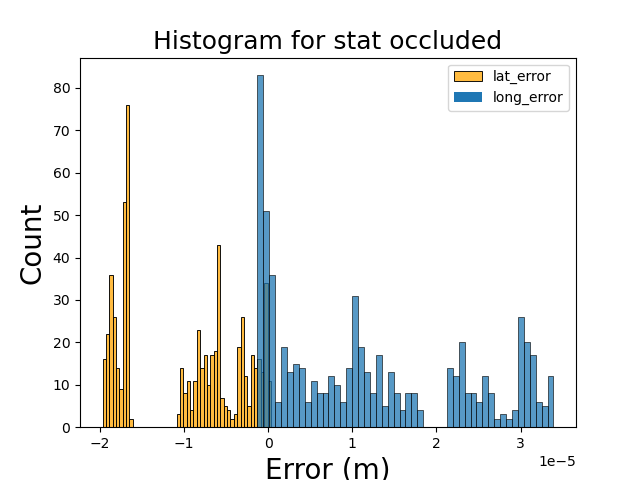
\includegraphics[scale = 0.5]{plot-Histogram for stat occluded.png}
\end{subfigure}
\begin{subfigure}{}
    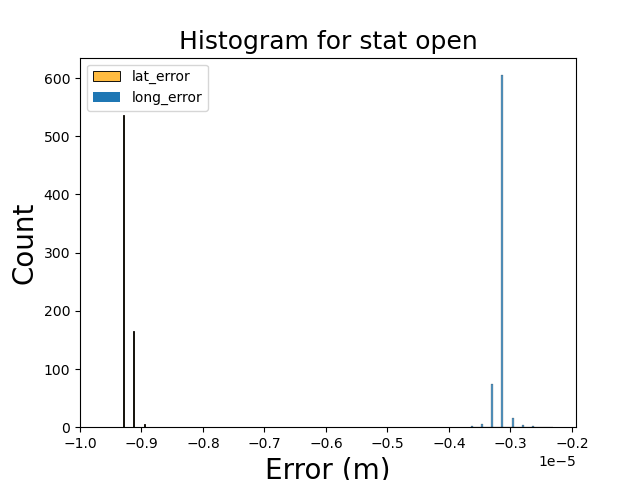
\includegraphics[scale = 0.5]{plot-Histogram for stat open.png}
\end{subfigure}
\caption{Histograms of error from known and measured data.}
\label{Fig2: Histograms}
\end{figure}
Although we can directly visualize the error from fig \ref{Fig 1: UTM Easting vs UTM Northing Scatterplots.} that the noise/error is a tightly packed \textbf{Gaussian model} with a significantly lower value of $\sigma$ for stationary open positions (not for occluded data due to several multipath). To better explain this fig \ref{Fig2: Histograms} are used. \textbf{The occluded region was more occluded than required which caused this sparely packed scatterplot and histogram}. To better analyze this mathematical steps like \textit{Chi-square methods} can be performed for identifying normality in data.
\section{Why is this distribution different from the one collected in Lab 1.}
We used standard GPS pucks in Lab 1 for data collection. They don't use differential data  collection and correction to output a more accurate and precise location, whereas RTK does. To put this into perspective if we know the location of any place or person then based on that we can relatively calculate our position. This is what RTK modules do.\\
Standard GPS modules use \textit{Trilateration} for data collection. Whereas the base also collects the \textit{Ephemeris} data from satellite and performs correction. The corrections include the removal of atmospheric errors, satellite orbit errors, and receiver noise. As a result, the position calculated by the rover receiver using the corrected measurements is much more accurate than that of non-RTK GPS. Hence causing the distribution to change from \textbf{\textit{Lab 1}}.
\section{Comparing moving datasets}
Moving datasets from open and occluded had the same output. In our case, the moving occluded data had a fixed quality of \textbf{5 - RTK Float} whereas the same for moving open was \textbf{4 - RTK Fixed} but this small change in quality did not create any drastic change in output. Although the floating quality is the first level of positioning accuracy and fixed is the second and most accurate, in reality, this did not create any significant change for us.
Although we cannot perform linear regression on such a dataset as we moved in a rectangular pattern, to compare it with a GPS puck we did it and calculated the RMSE of that line fit.
\begin{figure}[h]
    \centering
    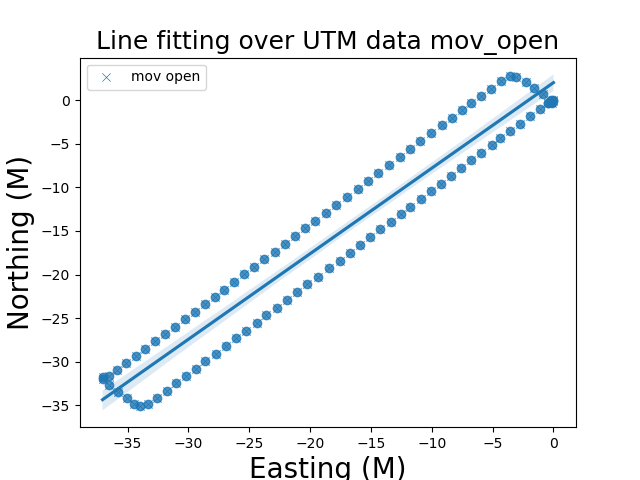
\includegraphics[scale = 0.3]{plot-Line fitting over UTM data mov_open.png}
    \caption{Linefit over moving open data}
    \label{fig: Linefit over moving open data}
\end{figure}
\begin{center}
    \begin{tabularx}{0.8\textwidth} { 
  | >{\centering\arraybackslash}X
  | >{\centering\arraybackslash}X |}
 \hline
 \textbf{RMSE for occluded moving data} & 5.228\\
 \hline
 \textbf{RMSE for open moving data} & 3.097\\
\hline
\end{tabularx}
\end{center}
The above RMSE is significantly less than what we got in Lab 1 i.e \textbf{24 for occluded} and \textbf{7 for open}.
\section{Compare stationary datasets}
As mentioned above the GNSS Quality account for the accuracy of the data collected. It is evident from fig \ref{Fig 1: UTM Easting vs UTM Northing Scatterplots.} for stationary occluded data that the data jumped from one position to another and there is a significant change in between, this is because while data collection for a brief amount of time we received GNSS fix quality as 1 and 2. This change \textbf{from 4 to 1 and 2} caused the data to jump causing significant errors.
\section{Experimental data analysis}
Below are the plots for altitude vs time for stationary datasets. The above-mentioned reasons for stationary occluded data collection also occurred for altitude. That jumps of GNSS fixed quality caused the output of altitude with and without correction. \textbf{This jump clearly shows the importance of RTK-based GPS sensors.} Although there is no true value of altitude we cannot compare which jump is with fixed quality and which with float quality but the difference shows how much correction the GPS needs to correct its position.
\begin{figure}[h]
    \centering
    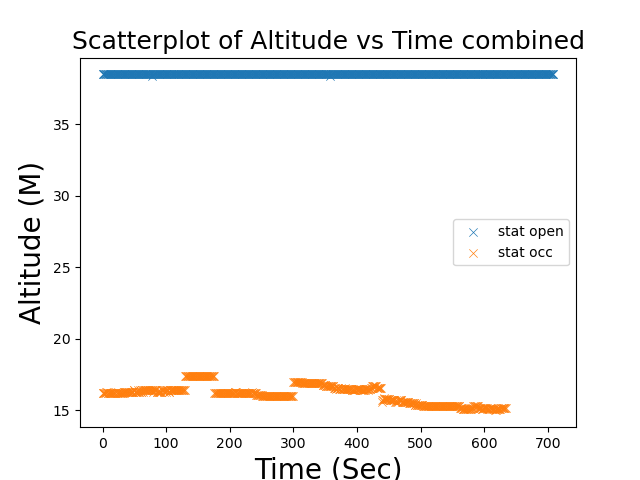
\includegraphics[scale = 0.4]{plot-Scatterplot of Altitude vs Time combined.png}
    \caption{Altitude vs Time}
    \label{fig: Altitude vs Time}
\end{figure}
\end{document}

